\label{section:edge-area-chapter}
As the section before, we want now to show extensions where we split the surface of the triangle mesh likewise into regions around  edges and we draw all pixels in these regions with the same color (see Figure \ref{fig:edge-area}). This results in rhombus-shaped areas with constant color around each edge.

\begin{figure}[H]
    \centering
    \minipage[b]{.5\linewidth}
    \centering
    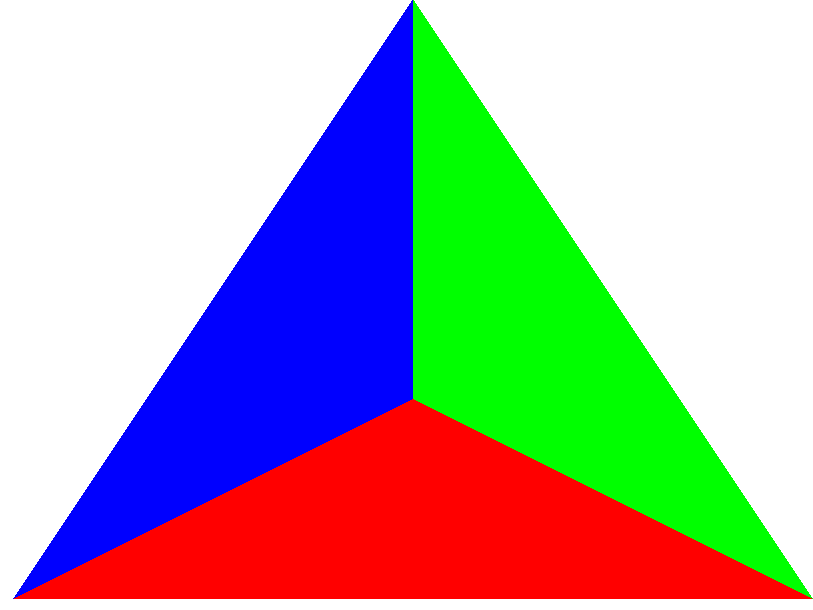
\includegraphics[scale=0.15]{images/min.png}
    \caption{Min diagram}\label{fig:min-diagram}
    \endminipage\hfill
    \minipage[b]{.5\linewidth}
    \centering
    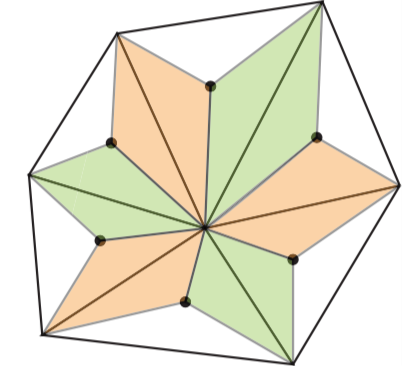
\includegraphics[scale=0.6]{images/edge-area.png}
    \caption{Region around an edge}\label{fig:edge-area}
    \endminipage
\end{figure}

\subsection{Min diagram - Edge area} \label{section:min-diagram}
For each point in a triangle, we can easily determine its closest edge, which we use as a cue for coloring.
A different approach from interpolating, can be found coloring vertex areas based on the minimum barycentric coordinate.
The color is given by the region farthest from a vertex (Fig. \ref{fig:min-diagram}, Pseudocode \ref{appendix:min-diagram}).

\subsection{Mean Curvature} \label{section:edge-struct} \label{section:mc-curvature}
Access to mesh edges requires to set up a list of edges over triangles. To avoid redundant datas we have decided to use the convention that an edge would be count only if it goes from a lower to higher vertex. An edge structure looks like the one in the pseudocode \ref{Pseudocode:edge}, where index\_v1 and index\_v2 are the indexes vertices, norm\_edge is the length of edge, n1 and n2 are the normals of triangles, cot\_alpha and cot\_beta are the cotangents of opposite angles to the edge, area\_t1 and area\_t2 are the areas of triangles.

\subsection{Constant Mean Curvature}
\textit{Constant mean Curvature} returns a constant color around each edge (See Fig. \ref{fig:armadillo-mean-edge}). It first calculate the mean curvature for each edge:
$$H(E) = || E|| (\theta_E /2)$$
where $\theta_E$ is the angle between the two normals of $T_1$ and $T_2$ (See Fig. \ref{fig:mean-edge}).
\begin{figure}[H]
    \centering
    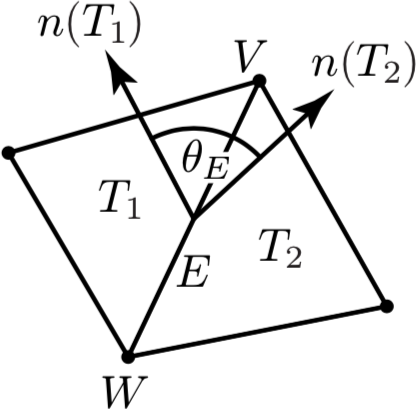
\includegraphics[scale=0.6]{images/mean-edge-theta.png}
    \caption{The dihedral angle $\theta_E$ at a mesh edge $E$ is the angle between the normals of the adjacent triangles. \cite{geometryprocessing}}\label{fig:mean-edge}
\end{figure}
The mean curvature for each vertex $V$ of a mesh is defined as:
$$H(E) = \frac{1}{2\mathcal{A}_{Barycentre}} \sum_{i = 1}^n ||E_i||(\theta_E/2)$$
This value is then normalized since it is an integral value. Every value is then mapped to positive or negative curvature, depending if the mesh at this edge is convex or concave, testing the $3D$ determinant of the 3-by-3 matrix $M = [e, n_1, n_2]$ with those three vectors as
columns ($e$ is the edge $[W, V]$, $n_1$ is the normal of $T_1$ and $n_2$ is the normal of $T_2$). If $det(M) > 0$ then the mesh is convex at $[W, V]$ and the mean curvature would be positive, else the mesh is concave and the mean curvature would be negative. This technique of edge flat shading represents an alternative to the classic triangle flat shading.

\begin{figure}[!h]
    \centering
    \minipage[b]{.5\linewidth}
    \centering
    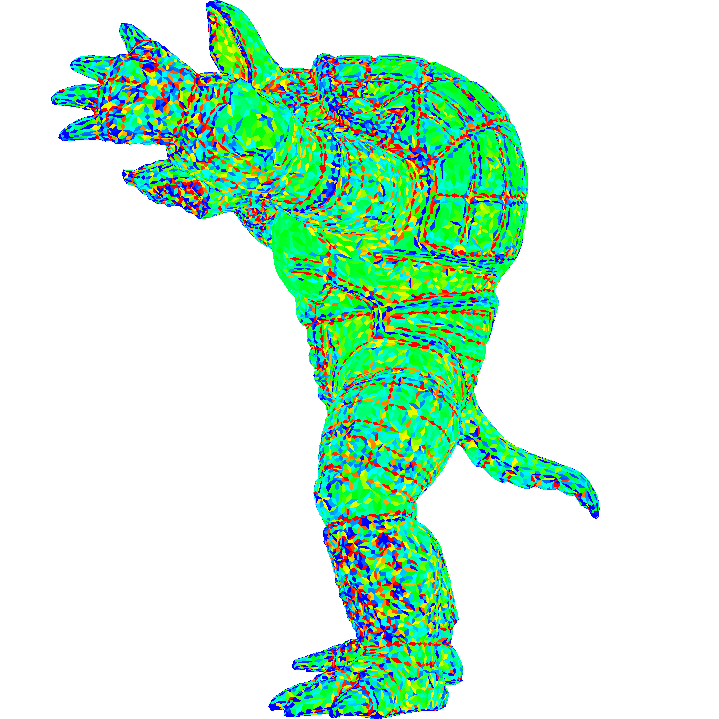
\includegraphics[scale=0.5]{images/mean-curvature-edge.png}
    \endminipage\hfill
    \minipage[b]{.5\linewidth}
    \centering
    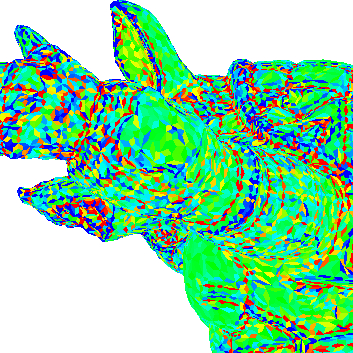
\includegraphics[scale=1.0]{images/mean-curvature-edge-detail.png}
    \endminipage
    \caption{Constant mean curvature} \label{fig:armadillo-mean-edge}
\end{figure}

\subsection{Gouraud Mean Curvature}
\textit{Gouraud mean Curvature} returns an interpolated color around each vertex. The main idea is to calculate the mean curvature $H(V)$ for each vertex $V$. In a mesh, every edge has two opposite angles (let us denominate these with $\alpha$ and $\beta$), the mean curvature per vertex is defined as:
$$H(V) = \frac{1}{2\mathcal{A}_{Mixed}} \sum_{i=1}^{n}(\cot \alpha_i + \cot \beta_i) (V - V_i)$$
where $V_i$ is one of the endpoints of the edge $E_i$ (see Fig. \ref{fig:mean-edge-cot}).
\begin{figure}[H]
    \centering
    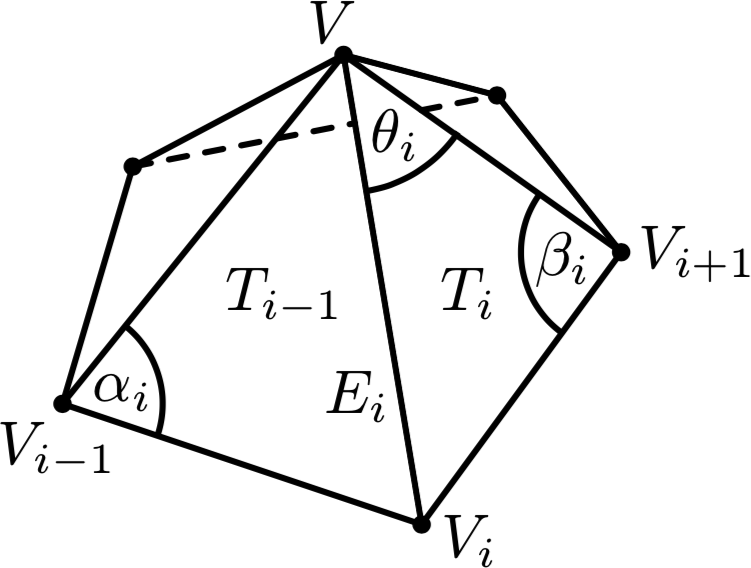
\includegraphics[scale=0.6]{images/mean-edge-cot.png}
    \caption{A vertex $V$ of a triangle mesh with neighbouring vertices $V_i$ and adjacent triangles $T_i$. The angle of $T_i$ at $V$ is denoted by $\theta_i$ and the angles opposite the edge $E_i$ by $\alpha_i$ and $\beta_i$. \cite{geometryprocessing}}\label{fig:mean-edge-cot}
\end{figure}

These values are then interpolated using the automatic OpenGL interpolation resembling the classic Gouraud shading (see Fig. \ref{fig:armadillo-mean-vertex}).

\begin{figure}[!h]
    \centering
    \minipage[b]{.5\linewidth}
    \centering
    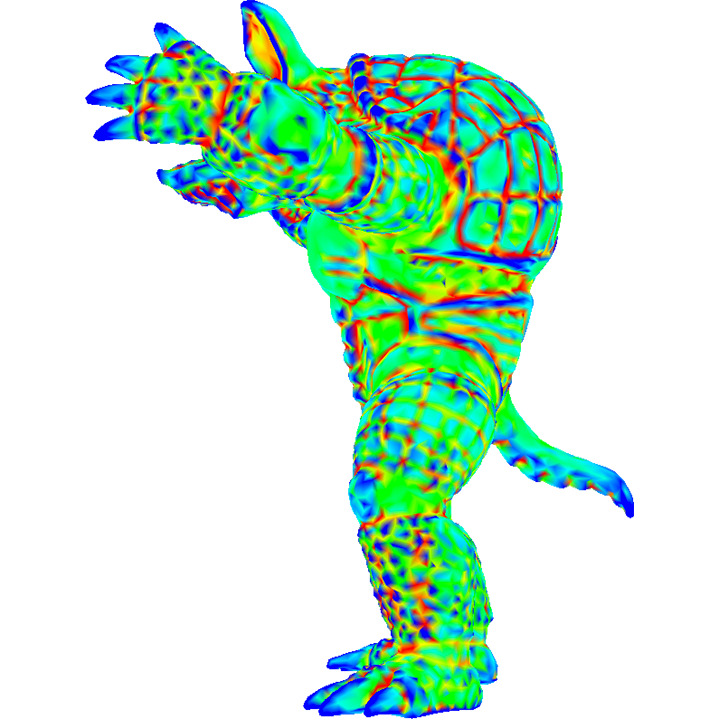
\includegraphics[scale=0.24]{images/mean-curvature-vertex.png}
    \endminipage\hfill
    \minipage[b]{.5\linewidth}
    \centering
    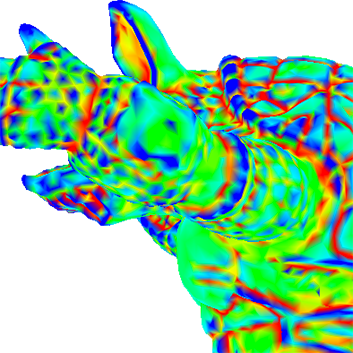
\includegraphics[scale=0.5]{images/mean-curvature-vertex-detail.png}
    \endminipage
    \caption{Gouraud mean curvature} \label{fig:armadillo-mean-vertex}
\end{figure}


\subsection{Evaluation and Comparison between constant mean curvature and gouraud mean curvature}
\textit{Constant mean curvature} is a curvature per
edge that return a constant color around each edge
using the min diagram algorithm. The result is a noisy and sharped mesh that emphasizes edge. This visualization could be helpfull to show the quality of mesh triangulation and flows around surfaces. These last are observable because edge are directed allowing the user to better analyze curvatures (see Fig. \ref{fig:armadillo-mean-edge}). \textit{Gouraud mean curvature}, on the other hand, return blurry meshes than the ones obtained with  \textit{Gouraud Gaussian curvature}. This smooth is caused by the fact that we are averaging per vertex, mean curvature would be calculated per edge but in this case, we had applied it on vertices opposite to edges, this result in a losing of data (see Fig. \ref{fig:armadillo-mean-vertex}).
\begin{figure}[!h]
    \centering
    \minipage[b]{.5\linewidth}
    \centering
    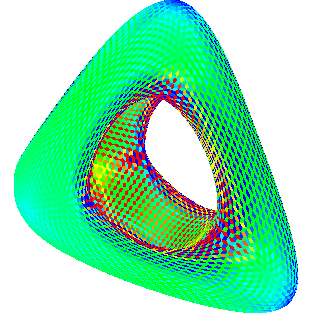
\includegraphics[scale=0.7]{images/genus-mce.png}
    \endminipage\hfill
    \centering
    \minipage[b]{.5\linewidth}
    \centering
    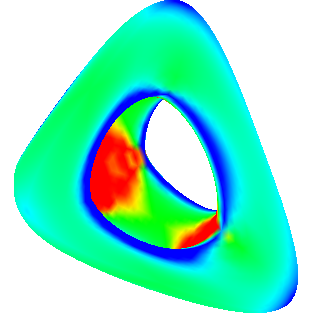
\includegraphics[scale=0.7]{images/genus-mcv.png}
    \endminipage\hfill
    \minipage[b]{.5\linewidth}
    \centering
    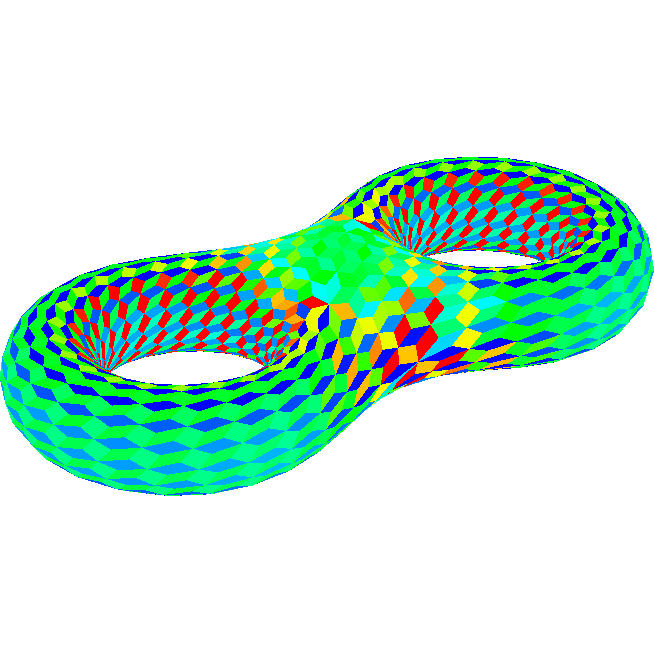
\includegraphics[scale=0.45]{images/eight-mce.png}
    \endminipage\hfill
    \centering
    \minipage[b]{.5\linewidth}
    \centering
    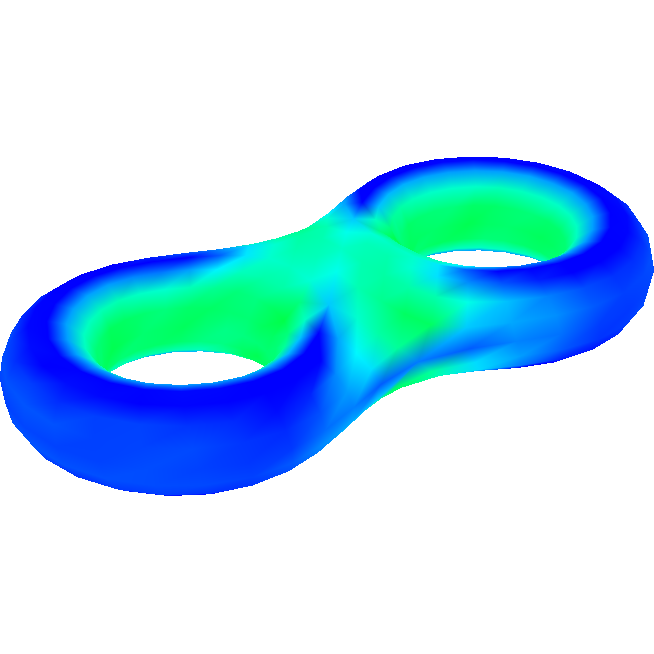
\includegraphics[scale=0.45]{images/eight-mcv.png}
    \endminipage\hfill
    \centering
    \minipage[b]{.5\linewidth}
    \centering
    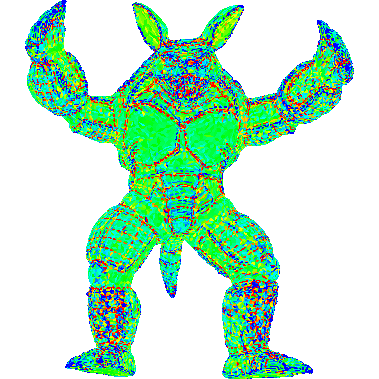
\includegraphics[scale=0.7]{images/armadillo-mce.png}
    \endminipage\hfill
    \centering
    \minipage[b]{.5\linewidth}
    \centering
    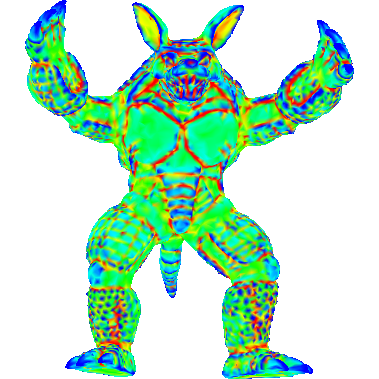
\includegraphics[scale=0.7]{images/armadillo-mcv.png}
    \endminipage\hfill
    \minipage[b]{.5\linewidth}
    \centering
    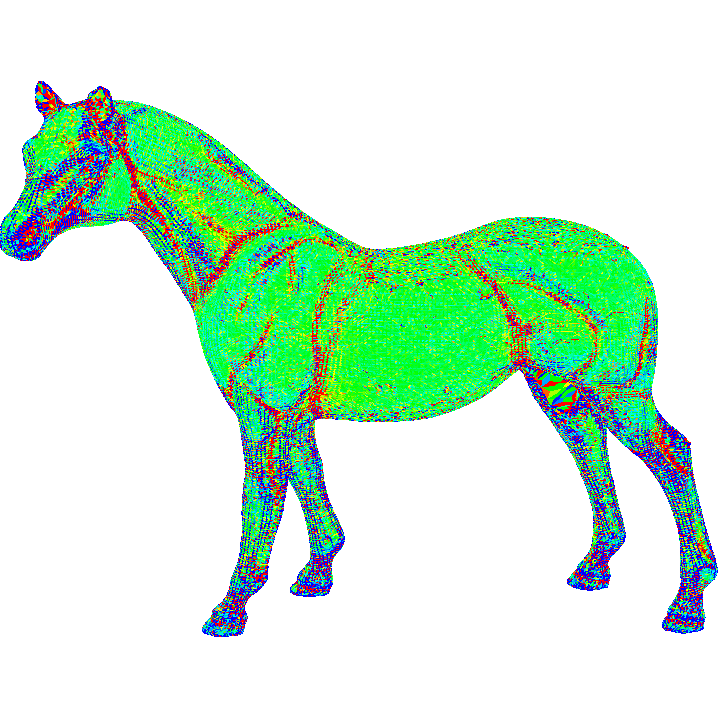
\includegraphics[scale=0.42]{images/horse-mce.png}
    \endminipage\hfill
    \centering
    \minipage[b]{.5\linewidth}
    \centering
    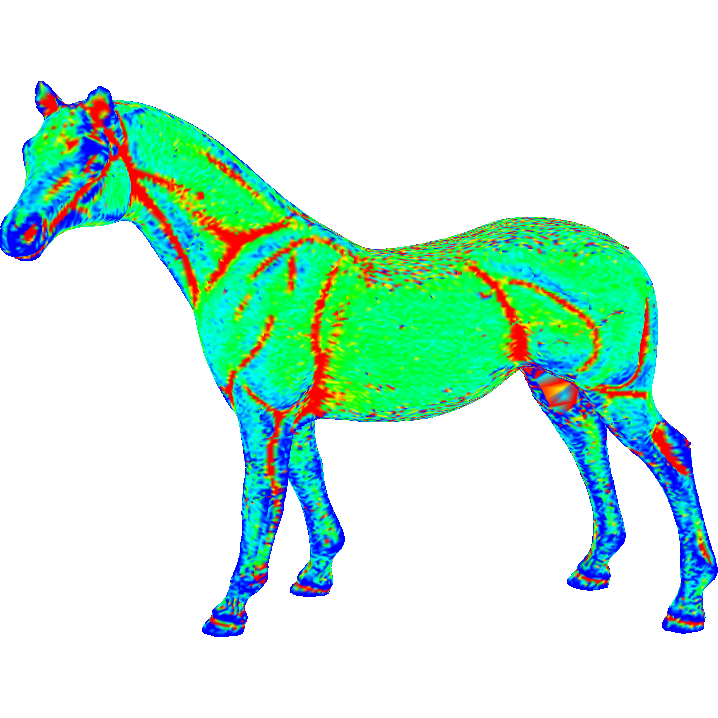
\includegraphics[scale=0.42]{images/horse-mcv.png}
    \endminipage\hfill
    \caption{On the left: Mean curvature per edge. On the right: Gouraud mean curvature.}
    \label{fig:comparison-mce-mcv}
\end{figure}